\documentclass[a4paper,12pt]{article}
\usepackage{amsmath,amssymb}
\usepackage{graphicx}
\usepackage{scaladefs}
\usepackage{scalit}
\usepackage{fancyhdr}
\pagestyle{fancy}
\lhead{\today}
\rhead{tangle/tangle.nw}
\begin{document}
\section{How to extract source code from a literate program}
\texttt{tangle} is the tool that extracts source code from a given literate
program. For this extraction, we base ourselves on the stream of blocks
generated in the file \texttt{markup/blocks.nw}

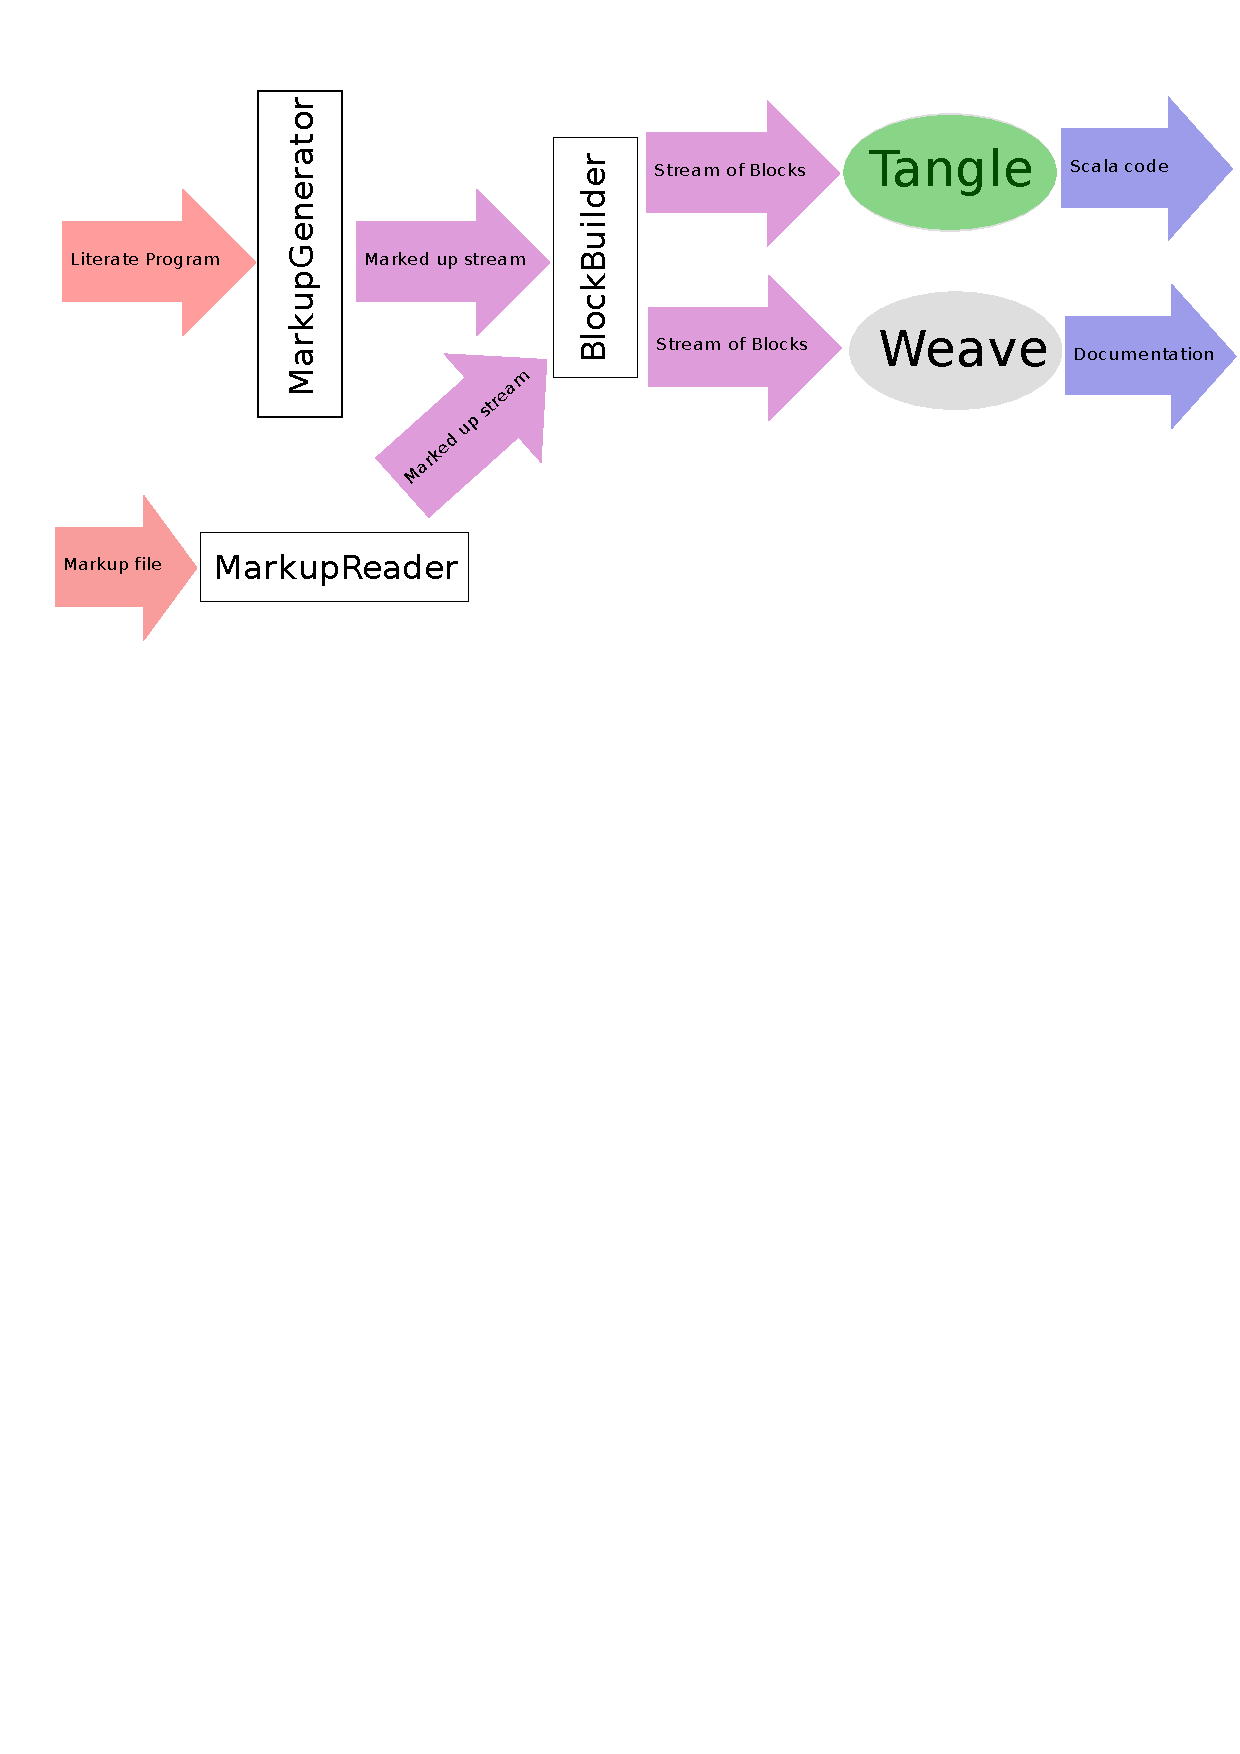
\includegraphics[width=10cm,viewport=310 710 600 800,clip]{images/tangle}

\subsection{Overview}
Tangle will first extract a map of code blocks, from which it will
output the sources in the right format the routines for output are
directly associated with the map and will be explained in section
\ref{puzzle}.

$\left<\mbox{\emph{*}}\right>\equiv$
\begin{program}{\vem package}~scalit.tangle
\\{\vem import}~markup.\_
\\[0.5em]$<$code~chunks$>$
\\[0.5em]$<$puzzle~code~chunks~together$>$
\\[0.5em]$<$output~the~source$>$
\\[0.5em]\end{program}


\label{puzzle}\subsection{Puzzling code blocks together}
\subsubsection{Code chunks}
While the block generator already provides us with a stream of
blocks, several of these might be describing the same code chunk.
So a pointer to the next code block describing this chunk has to be
provided. We do this using an \texttt{Option}:

$\left<\mbox{\emph{code chunks}}\right>\equiv$
\begin{program}{\vem case}~{\vem class}~CodeChunk$($bn\,{\rm :}~Int,~ln\,{\rm :}~Int,
\\~~~~~~~~~~~~~~~~~~~~~~cont\,{\rm :}~Stream$[$Line$]$,bname\,{\rm :}~String,
\\~~~~~~~~~~~~~~~~~~~~~~next\,{\rm :}~Option$[$CodeChunk$]$$)$~{\vem extends}
\\CodeBlock$($bn,ln,cont,bname$)$~{\small\{}
\\~~~~
\\~~~~{\vem import}~StringRefs.\_
\\[0.5em]\end{program}\classdefinition{CodeChunk}
\valuedefinition{CodeChunk}{bn }
\valuedefinition{CodeChunk}{ln }
\valuedefinition{CodeChunk}{cont }
\valuedefinition{CodeChunk}{bname }
\valuedefinition{CodeChunk}{next }



The append method will be useful when we will actually construct
the chunks.

$\left<\mbox{\emph{code chunks}}\right>+\equiv$
\begin{program}~~~~{\vem def}~append$($that\,{\rm :}~CodeBlock$)${\rm :}~CodeChunk~=~next~{\vem match}~{\small\{}
\\~~~~~~~~{\vem case}~None~$\Rightarrow$
\\~~~~~~~~~~~~CodeChunk$(${\vem this}.blocknumber,
\\~~~~~~~~~~~~~~~~~~~~~~~~~~~~~~~~{\vem this}.linenumber,
\\~~~~~~~~~~~~~~~~~~~~~~~~~~~~~~~~{\vem this}.content,
\\~~~~~~~~~~~~~~~~~~~~~~~~~~~~~~~~{\vem this}.blockname,
\\~~~~~~~~~~~~~~~~~~~~~~~~~~~~~~~~Some$($CodeChunk$($that.blocknumber,
\\~~~~~~~~~~~~~~~~~~~~~~~~~~~~~~~~~~~~~~~~that.linenumber,
\\~~~~~~~~~~~~~~~~~~~~~~~~~~~~~~~~~~~~~~~~that.content,
\\~~~~~~~~~~~~~~~~~~~~~~~~~~~~~~~~~~~~~~~~that.blockname,None$)$$)$$)$
\\~~~~~~~~{\vem case}~Some$($next$)$~$\Rightarrow$
\\~~~~~~~~~~~~CodeChunk$(${\vem this}.blocknumber,
\\~~~~~~~~~~~~~~~~~~~~~~~~~~~~~~~~{\vem this}.linenumber,
\\~~~~~~~~~~~~~~~~~~~~~~~~~~~~~~~~{\vem this}.content,
\\~~~~~~~~~~~~~~~~~~~~~~~~~~~~~~~~{\vem this}.blockname,
\\~~~~~~~~~~~~~~~~~~~~~~~~~~~~~~~~Some$($next~append~that$)$$)$
\\~~~~{\small\}}
\\[0.5em]\end{program}\methoddefinition{CodeChunk}{append}



With this linked-list-like definition in place, we can also redefine
the string reference form by simply appending the output of the next
element:

$\left<\mbox{\emph{code chunks}}\right>+\equiv$
\begin{program}~~~~{\vem override}~{\vem def}~stringRefForm$($codeChunks\,{\rm :}~Map$[$String,CodeBlock$]$$)${\rm :}
\\~~~~~~~~Stream$[$StringRef$]$~=~next~{\vem match}~{\small\{}
\\~~~~~~~~~~~~{\vem case}~None~$\Rightarrow$~{\vem super}.stringRefForm$($codeChunks$)$
\\~~~~~~~~~~~~{\vem case}~Some$($el$)$~$\Rightarrow$~Stream.concat$($
\\~~~~~~~~~~~~~~~~{\vem super}.stringRefForm$($codeChunks$)$,
\\~~~~~~~~~~~~~~~~el.stringRefForm$($codeChunks$)$$)$
\\~~~~~~~~{\small\}}
\\{\small\}}
\\[0.5em]\end{program}\methoddefinition{CodeChunk}{stringRefForm}



\subsubsection{A collection of chunks}
In a chunk collection, we accumulate chunks on in a map. Also
very important is the file name.

$\left<\mbox{\emph{puzzle code chunks together}}\right>\equiv$
\begin{program}{\vem import}~scala.collection.immutable.{\small\{}Map,HashMap{\small\}}
\\{\vem case}~{\vem class}~ChunkCollection$($cm\,{\rm :}~Map$[$String,CodeChunk$]$,
\\~~~~~~~~~~~~~~~~~~~~~~~~~~~~~~~~~~~~~~~~~~~~~~~~~~filename\,{\rm :}~String$)$~{\small\{}
\\[0.5em]~~~~{\vem import}~StringRefs.\_
\\[0.5em]\end{program}\classdefinition{ChunkCollection}
\valuedefinition{ChunkCollection}{cm }
\valuedefinition{ChunkCollection}{filename }



To get the stream of code is now as simple as calling
serialize. Flatten will convert it to a string.

$\left<\mbox{\emph{puzzle code chunks together}}\right>+\equiv$
\begin{program}~~~~{\vem def}~serialize$($chunkname\,{\rm :}~String$)${\rm :}~String~=
\\~~~~~~~~cm~get~chunkname~{\vem match}~{\small\{}
\\~~~~~~~~~~~~{\vem case}~None~$\Rightarrow$~error$($"Did~not~find~chunk~"~$+$~chunkname$)$
\\~~~~~~~~~~~~{\vem case}~Some$($el$)$~$\Rightarrow$~flatten$($el.stringRefForm$($cm$)$$)$
\\~~~~~~~~{\small\}}
\\[0.5em]\end{program}\methoddefinition{ChunkCollection}{serialize}



From the stream of blocks, we will receive the code blocks. We
will have to generate code chunks out of them.

$\left<\mbox{\emph{puzzle code chunks together}}\right>+\equiv$
\begin{program}~~~~{\vem def}~addBlock$($that\,{\rm :}~CodeBlock$)${\rm :}~ChunkCollection~=
\\~~~~~~~~cm~get~that.blockname~{\vem match}~{\small\{}
\\~~~~~~~~~~~~{\vem case}~None~$\Rightarrow$~ChunkCollection$($cm~$+$
\\~~~~~~~~~~~~~~~~$($that.blockname~$\rightarrow$
\\~~~~~~~~~~~~~~~~~~CodeChunk$($that.blocknumber,
\\~~~~~~~~~~~~~~~~~~~~~~~~~~~~~~~~~~~~that.linenumber,
\\~~~~~~~~~~~~~~~~~~~~~~~~~~~~~~~~~~~~that.content,
\\~~~~~~~~~~~~~~~~~~~~~~~~~~~~~~~~~~~~that.blockname,
\\~~~~~~~~~~~~~~~~~~~~~~~~~~~~~~~~~~~~None$)$$)$,filename$)$
\\~~~~~~~~~~~~{\vem case}~Some$($el$)$~$\Rightarrow$~ChunkCollection$($cm~$+$
\\~~~~~~~~~~~~~~~~$($that.blockname~$\rightarrow$
\\~~~~~~~~~~~~~~~~~~el.append$($that$)$$)$,filename$)$
\\~~~~~~~~{\small\}}
\\[0.5em]\end{program}\methoddefinition{ChunkCollection}{addBlock}



While adding one block is useful, we will want to do this
for a whole stream of blocks:

$\left<\mbox{\emph{puzzle code chunks together}}\right>+\equiv$
\begin{program}~~~~{\vem def}~addBlocks$($those\,{\rm :}~Stream$[$CodeBlock$]$$)${\rm :}~ChunkCollection~=
\\~~~~~~~~$($those~foldLeft~{\vem this}$)$~{\small\{}
\\~~~~~~~~~~~~$($acc\,{\rm :}~ChunkCollection,~n\,{\rm :}~CodeBlock$)$~$\Rightarrow$
\\~~~~~~~~~~~~~~~~acc.addBlock$($n$)$
\\~~~~~~~~{\small\}}
\\[0.5em]\end{program}\methoddefinition{ChunkCollection}{addBlocks}



Finally, we'll have to define how to output a string containing the
whole code. In a first step, we'll have to expand references:

$\left<\mbox{\emph{puzzle code chunks together}}\right>+\equiv$
\begin{program}~~~~{\vem def}~expandRefs$($str\,{\rm :}~Stream$[$StringRef$]$$)${\rm :}~Stream$[$RealString$]$~=
\\~~~~~~~~str~{\vem match}~{\small\{}
\\~~~~~~~~~~~~{\vem case}~Stream.empty~$\Rightarrow$~Stream.empty
\\~~~~~~~~~~~~{\vem case}~Stream.cons$($first,rest$)$~$\Rightarrow$
\\~~~~~~~~~~~~~~~~first~{\vem match}~{\small\{}
\\~~~~~~~~~~~~~~~~~~~~{\vem case}~r~@~RealString$($\_,\_,\_$)$~$\Rightarrow$
\\~~~~~~~~~~~~~~~~~~~~~~~~Stream.cons$($r,expandRefs$($rest$)$$)$
\\~~~~~~~~~~~~~~~~~~~~{\vem case}~BlockRef$($ref$)$~$\Rightarrow$
\\~~~~~~~~~~~~~~~~~~~~~~~~Stream.concat$($
\\~~~~~~~~~~~~~~~~~~~~~~~~~~~~expandRefs$($cm$($ref.blockname$)$.stringRefForm$($cm$)$$)$,
\\~~~~~~~~~~~~~~~~~~~~~~~~~~~~expandRefs$($rest$)$$)$
\\~~~~~~~~~~~~~~~~~~~~{\vem case}~other~$\Rightarrow$~error$($"Unexpected~string~ref\,{\rm :}~"~$+$~other$)$
\\~~~~~~~~~~~~~~~~{\small\}}
\\~~~~~~~~{\small\}}
\\[0.5em]~~~~{\vem def}~expandedStream$($chunkname\,{\rm :}~String$)${\rm :}~Stream$[$RealString$]$~=
\\~~~~~~~~cm~get~chunkname~{\vem match}~{\small\{}
\\~~~~~~~~~~~~{\vem case}~None~$\Rightarrow$~error$($"Did~not~find~chunk~"~$+$~chunkname$)$
\\~~~~~~~~~~~~{\vem case}~Some$($el$)$~$\Rightarrow$~expandRefs$($el.stringRefForm$($cm$)$$)$
\\~~~~~~~~{\small\}}
\\[0.5em]\end{program}\methoddefinition{ChunkCollection}{expandRefs}
\methoddefinition{ChunkCollection}{expandedStream}



After this expansion, the string form is quite easily made:

$\left<\mbox{\emph{puzzle code chunks together}}\right>+\equiv$
\begin{program}~~~~{\vem private}~{\vem def}~flatten$($str\,{\rm :}~Stream$[$StringRef$]$$)${\rm :}~String~=~{\small\{}
\\~~~~~~~~{\vem val}~sb~=~{\vem new}~StringBuffer
\\~~~~~~~~expandRefs$($str$)$~foreach~{\small\{}
\\~~~~~~~~~~~~{\vem case}~RealString$($content,\_,\_$)$~$\Rightarrow$~sb~append~content
\\~~~~~~~~{\small\}}
\\~~~~~~~~sb.toString
\\~~~~{\small\}}
\\{\small\}}
\\[0.5em]\end{program}\methoddefinition{ChunkCollection}{flatten}



With the chunk collection logic in place, we will often have to access
to the empty chunk collection of a particular file name:

$\left<\mbox{\emph{puzzle code chunks together}}\right>+\equiv$
\begin{program}{\vem case}~{\vem class}~emptyChunkCollection$($fn\,{\rm :}~String$)$
\\~~~~~~~~~~{\vem extends}~ChunkCollection$($Map$($$)$,fn$)$
\\[0.5em]\end{program}\classdefinition{emptyChunkCollection}
\valuedefinition{emptyChunkCollection}{fn }



 \subsection{The main program}
With serialize defined, we can now accomplish the task of printing
the tangled source to standard output. Under \texttt{util/commandline.nw},
we defined a class for command line parsing that will be used here.
At the moment, we print out everything to standard output, one chunk
collection after another.

The following options can be given to tangle:

\begin{description}
\item[-r chunkname] Tries to extract the chunk with the name \texttt{chunkname}
\end{description}

$\left<\mbox{\emph{output the source}}\right>\equiv$
\begin{program}{\vem object}~Tangle~{\small\{}
\\~~~~{\vem def}~main$($args\,{\rm :}~Array$[$String$]$$)$~=~{\small\{}
\\~~~~~~~~{\vem import}~util.LiterateSettings
\\[0.5em]~~~~~~~~{\vem val}~ls~=~{\vem new}~LiterateSettings$($args$)$
\\[0.5em]~~~~~~~~{\vem val}~chunksToTake~=~ls.settings~get~"$-$r"~{\vem match}~{\small\{}
\\~~~~~~~~~~~~{\vem case}~None~$\Rightarrow$~Nil
\\~~~~~~~~~~~~{\vem case}~Some$($cs$)$~$\Rightarrow$~cs.reverse
\\~~~~~~~~{\small\}}
\\[0.5em]~~~~~~~~{\vem val}~out~=~ls.output
\\[0.5em]~~~~~~~~chunksToTake~{\vem match}~{\small\{}
\\~~~~~~~~~~~~{\vem case}~Nil~$\Rightarrow$
\\~~~~~~~~~~~~~~~~ls.chunkCollections~foreach~{\small\{}
\\~~~~~~~~~~~~~~~~~~~~cc~$\Rightarrow$~out.println$($cc.serialize$($"$*$"$)$$)$
\\~~~~~~~~~~~~~~~~{\small\}}
\\[0.5em]\end{program}\objectdefinition{Tangle}
\methoddefinition{Tangle}{main}



If we have specified some chunks to extract, we iterate over all the files
that we are given, extracting the specific chunk.

$\left<\mbox{\emph{output the source}}\right>+\equiv$
\begin{program}~~~~~~~~~~~~{\vem case}~cs~$\Rightarrow$
\\~~~~~~~~~~~~~~~~cs~foreach~{\small\{}
\\~~~~~~~~~~~~~~~~~~~~chunk~$\Rightarrow$
\\~~~~~~~~~~~~~~~~~~~~~~~~ls.chunkCollections~foreach~{\small\{}
\\~~~~~~~~~~~~~~~~~~~~~~~~~~~~cc~$\Rightarrow$
\\~~~~~~~~~~~~~~~~~~~~~~~~~~~~~~~~{\vem try}~{\small\{}
\\~~~~~~~~~~~~~~~~~~~~~~~~~~~~~~~~~~~~out.println$($cc.serialize$($chunk$)$$)$
\\~~~~~~~~~~~~~~~~~~~~~~~~~~~~~~~~{\small\}}~{\vem catch}~{\small\{}
\\~~~~~~~~~~~~~~~~~~~~~~~~~~~~~~~~~~~~{\vem case}~e~$\Rightarrow$~$($$)$
\\~~~~~~~~~~~~~~~~~~~~~~~~~~~~~~~~{\small\}}
\\~~~~~~~~~~~~~~~~~~~~~~~~{\small\}}
\\~~~~~~~~~~~~~~~~{\small\}}
\\~~~~~~~~{\small\}}
\\~~~~{\small\}}
\\{\small\}}
\end{program}


\end{document}


